\section{Method}
\label{sec:method}

In this section we describe how we calculate full 3D velocities for stars in
the Kepler field.
Around 1 in 2 stars in the Kepler field have an RV from either Gaia, LAMOST,
or APOGEE.
For these \nrv\ stars we calculated 3D velocities using the {\tt coordinates}
library of {\tt astropy} \citep{astropy2013, astropy2018}.
This library performs a series of matrix rotations and translations to convert
stellar positions and velocities in equatorial
% , or International Celestial Reference System (ICRS)
coordinates into positions and velocities in Galactocentric coordinates.
In other words, it converts positions, proper motions, parallaxes/distances,
and RVs into \x, \y, \z, \vx, \vy, \vz.
For stars {\it without} RVs we inferred their velocities by marginalizing over
their RVs using the method described below.

% It has been demonstrated that the dispersion in vertical velocity, \vz, of a
% population of stars increases with the age of that population,
% \citep[\eg][]{stromberg1946, wielen1977, nordstrom2004, holmberg2007,
% holmberg2009, aumer2009, casagrande2011, ting2019, yu2018}.
% Most AVRs are calibrated using velocities in Galactocentric coordinates, \vx,
% \vy\ and \vz, which can only be calculated with full 6-D position and velocity
% information, \ie\ proper motions, position and radial velocity.
% In \citet{angus2020} we explored rotational evolution using velocity
% dispersion as an age proxy, however we used velocity in the direction of
% Galactic latitude, \vb, instead of \vz.
% This is because \vb\ can be calculated without an RV measurement but is a
% close approximation to \vz\ for \kepler\ stars due to the orientation of the
% Kepler field.
% The \kepler\ field lies at low Galactic latitudes, ($\sim 5-20$\degrees), so
% the ${\bf z}$-direction is similar to the ${\bf b}$-direction for \kepler\
% stars.
% However, even at such low latitudes, kinematic ages calculated with \vb\
% instead of \vz\ are likely to be systematically larger because of mixing
% between \vz, \vx\ and \vy.
% A direct measurement or precise estimate of \vz\ is necessary to calculate
% accurate kinematic ages.

\subsection{Inferring 3D velocities (marginalizing over missing RV
measurements)}
\label{sec:inference}

% Three-dimensional velocities in galactocentric coordinates: \vx, \vy, and \vz\
% can only be directly computed via a transformation from 3D velocities in
% another coordinate system, like the equatorial coordinates provided by \gaia:
% \mura, \mudec, and RV.
% For stars with no measured RV in \gaia\ DR2, \vx, vy, and \vz\ can still be
% inferred from positions and proper motions alone, by marginalizing over
% missing RV measurements.
For each star in our sample without an RV measurement, we inferred \vx, \vy,
and \vz\ from the 3D positions -- RA (\ra), dec (\dec), and parallax
(\parallax), and 2D proper motions (\mura\ and \mudec) provided in the \gaia\
EDR3 catalog \citep{gaia_edr3}.
We also simultaneously inferred distance (instead of using inverse-parallax)
to model velocities \citep[see \eg][]{bailer-jones2015, bailer-jones2018}.

Using Bayes rule, the posterior probability of the velocity parameters given
the Gaia data can be written:
\begin{equation}
    p({\bf v_{xyz}}, D | \mu_{\alpha}, \mu_{\delta}, \alpha, \delta, \pi) =
    p(\mu_{\alpha}, \mu_{\delta}, \alpha, \delta, \pi | {\bf v_{xyz}}, D)
    p({\bf v_{xyz}}) p(D),
\end{equation}
where $D$ is distance and ${\bf v_{xyz}}$ is the 3D vector of velocities.
To evaluate the likelihood function, our model predicts observable data from
model parameters, \ie\ it converts \vx, \vy\, \vz\ and $D$ to \pmra, \pmdec\
and \parallax.
In the first step of the model evaluation, cartesian coordinates, \x, \y, and
\z\, are calculated from \ra, \dec, and $D$ by applying a series of matrix
rotations, and a translation to account for the Solar position.
The cartesian Galactocentric velocity parameters, \vx, \vy, and \vz, are then
converted to equatorial coordinates, \pmra\ and \pmdec\ via another rotation.
The posterior PDFs of the parameters \vx, \vy, \vz, and $\ln(D)$ are sampled
by evaluating this model over a range of parameter values which are chosen by
via the No U-Turns Sampler (NUTS) algorithm in {\tt PyMC3}.
At each set of model parameters the likelihood is calculated via a Gaussian
likelihood function, and multiplied by a prior (described below) to produce
the posterior probability: the probability of those model parameters given the
data.

For computational efficiency, we used {\tt PyMC3} to sample the posterior PDFs
of stellar velocities \citep{pymc3}.
This required that we rewrite the {\tt astropy} coordinate transformation code
using {\tt numpy} and {\tt Theano} \citep{numpy, theano}.
The series of rotations and translations required to convert from equatorial
to Galactocentric coordinates is described in the astropy
documentation\footnote{
    https://docs.astropy.org/en/stable/coordinates/galactocentric.html }.
For each star in the \kepler\ field, we explored the posteriors of the four
parameters, \vx, \vy, \vz, and $\ln(D)$ using the {\it PyMC3} No U-Turn
Sampler (NUTS) algorithm, and the {\tt exoplanet} \python\ library
\citep{exoplanet}.
We tuned the {\it PyMC3} sampler for 1500 steps, with a target acceptance
fraction of 0.9, then ran four chains of 1000 steps for a total of 4000 steps.
This resulted in a $\hat{r}$-statistic (the ratio of intra-chain to
inter-chain variance) of around unity, indicating convergence.
Using PyMC3 made this inference procedure exceptionally fast -- taking just a
few seconds per star on a laptop.

\subsection{The prior}
\label{sec:prior}

As mentioned previously, the positioning of the \kepler\ field at low Galactic
latitude allows \vz\ to be well-constrained from proper motion measurements
alone.
This also happens to be the case for \vx, because the direction of the
\kepler\ field is almost aligned with the \y-axis of the Galactocentric
coordinate system and is almost perpendicular to both the \x\ and \z-axes (see
figure \ref{fig:kepler_field}).
For this reason, the \y-direction is similar to the radial direction for
observers near the Sun, so \vy\ will be poorly constrained for \kepler\ stars
without RV measurements.
On the other hand, \vx\ and \vz\ are almost perpendicular to the radial
direction and can be precisely inferred with proper motions alone.
\begin{figure}[ht!]
\caption{
\x, \y\ and \z\ positions of stars observed by \kepler, showing the
    orientation of the \kepler\ field.
The direction of the field is almost aligned with the \y-axis and almost
    perpendicular to the \x\ and \z-axes, which is why \vx\ and \vz\ can be
    tightly constrained for \kepler\ stars without RVs, but \vy\ cannot.
}
  \centering
    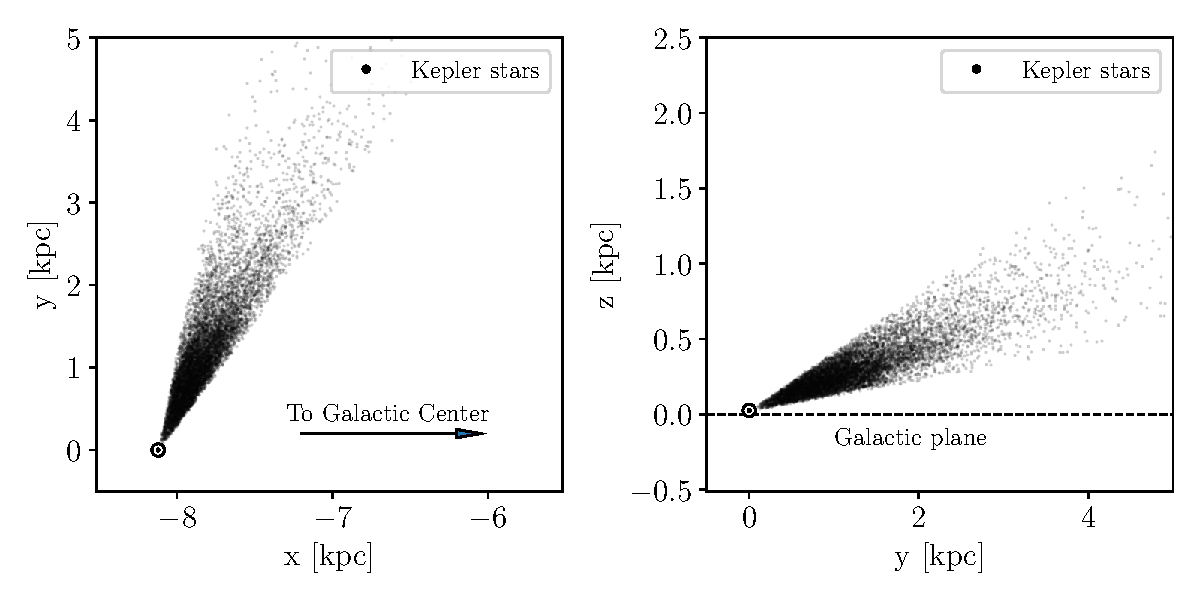
\includegraphics[width=.7\textwidth]{kepler_field}
\label{fig:kepler_field}
\end{figure}

We constructed a multivariate Gaussian prior PDF over distance and 3D velocity
using the Kepler targets {\it which have RV measurements}.
We calculated the means and covariances of the \vx, \vy, \vz\ and $\ln(D)$
distributions of stars with measured RVs and then used these means and
covariances to construct a multivariate Gaussian prior over the velocity and
distance parameters for stars {\it without} RVs.
Velocity outliers greater than 3-$\sigma$ were removed before calculating the
means and covariances of the distributions.
The distance and velocity distributions of Kepler targets with RVs are
displayed in figure \ref{fig:prior_distributions_2D}.
These are the distributions we used to construct the prior.
The 2-$\sigma$ contour of the multivariate Gaussian prior is shown in each
panel as a black ellipse.
\begin{figure}[ht!]
\caption{
The velocity and distance distributions for stars with RV measurements,
    used to construct a multivariate Gaussian prior over velocity and
    distance parameters for stars {\it without} RVs.
1 and 2-$\sigma$ contours are shown in red.
}
  \centering
    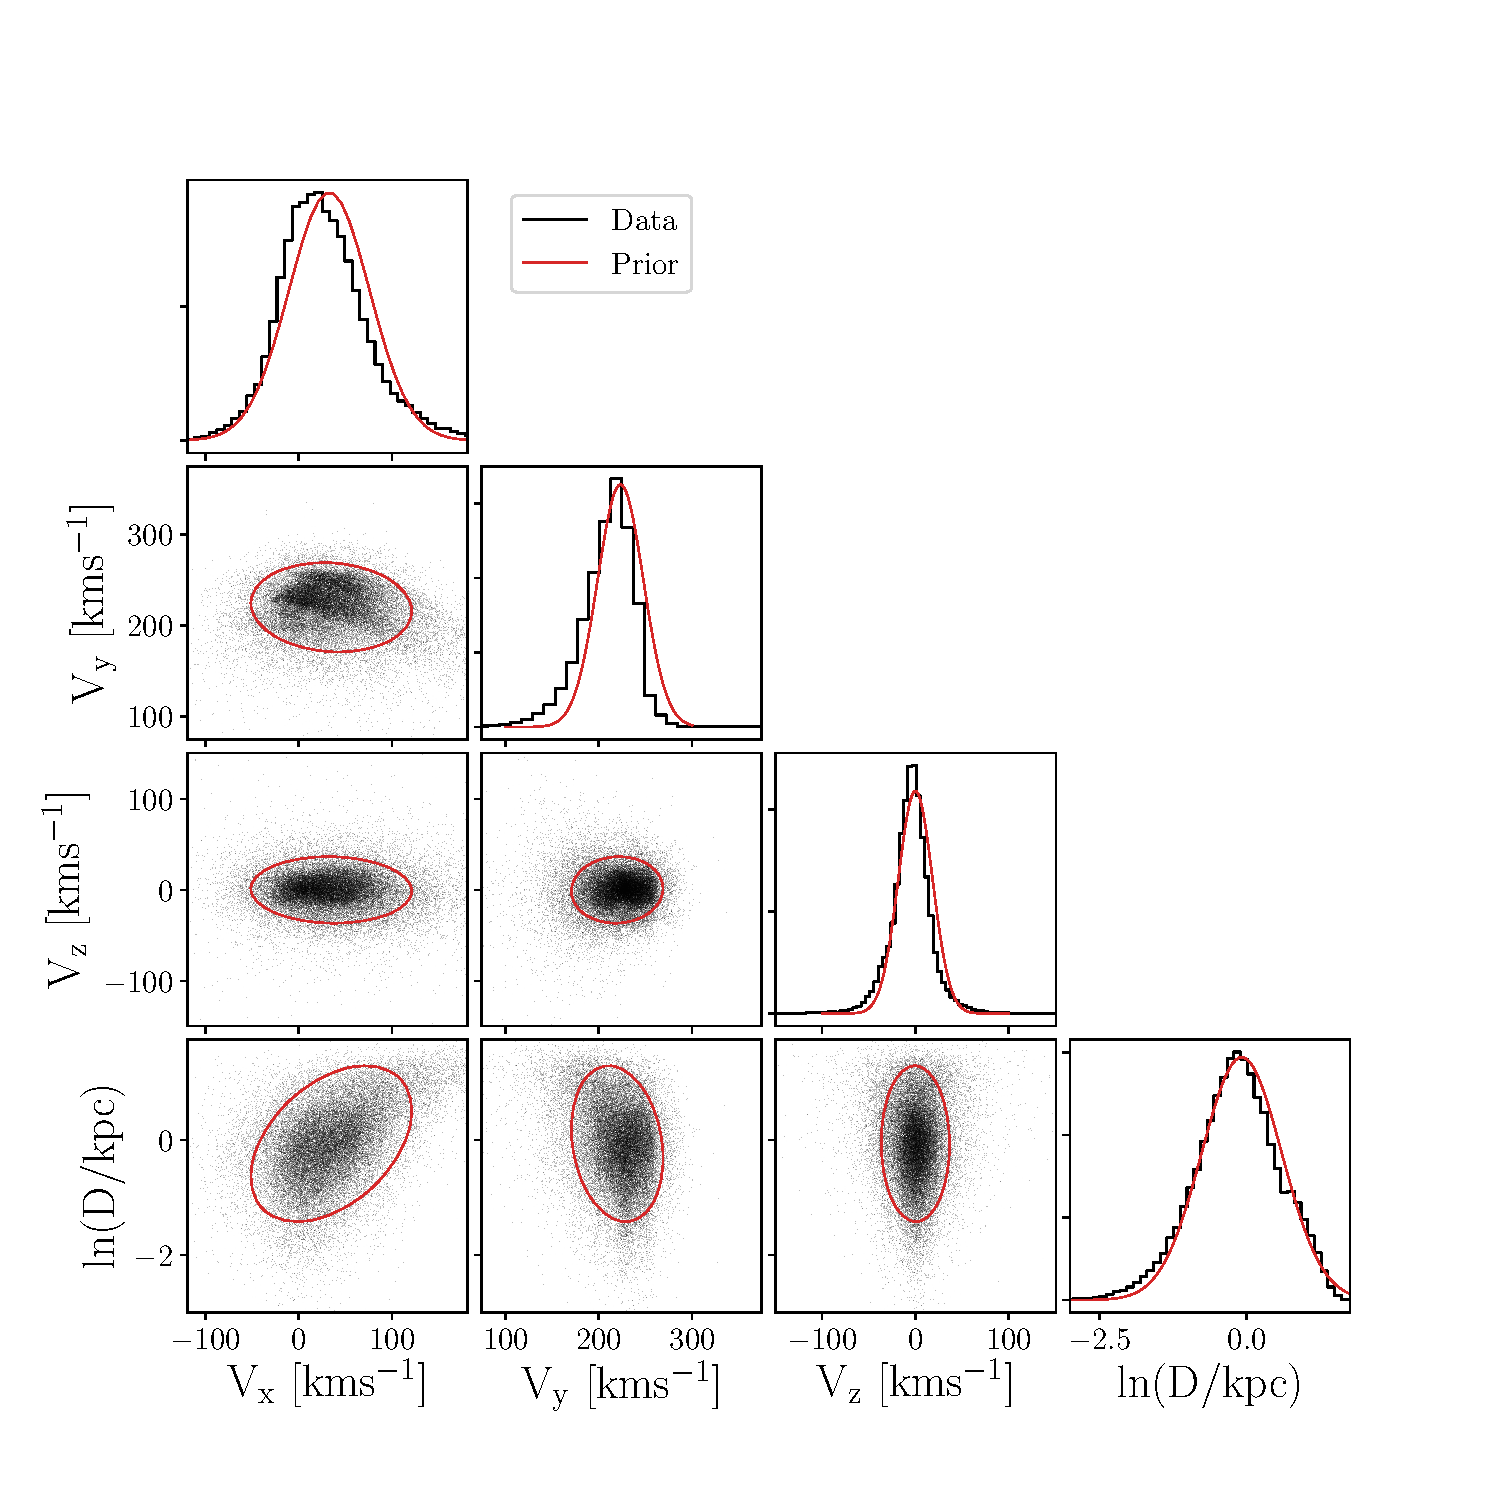
\includegraphics[width=.8\textwidth]{prior_distributions_2D}
\label{fig:prior_distributions_2D}
\end{figure}

Our goal was to infer the velocities of stars {\it without} RV measurements
using a prior calculated from stars {\it with} RV measurements.
However, stars with and without RVs are likely to be quite different
populations, determined by the Gaia, LAMOST and APOGEE selection functions.
In particular, stars without RV measurements are more likely to be fainter,
less luminous, cooler and potentially older.
Figure \ref{fig:CMD} shows the populations of stars with and without RVs on
the CMD -- stars with RVs are more likely to be upper-main-sequence and red
giant stars, and stars without RVs are more likely to be mid and lower
main-sequence dwarfs.
% Lower-mass stars are, on average, older, and have larger velocity dispersions,
% plus stars in different locations in the Galaxy have different orbital
% velocities.
For this reason, a prior based on the velocity distributions of stars {\it
with} RVs will not necessarily reflect the velocities of those without.
% However, given that \vx\ and \vz\ are strongly informed by proper motion
% measurements, and therefore likely to be relatively prior-insensitive, the
% prior may not significantly impact our final vertical velocities.

We tested the influence of the prior on the velocities we inferred.
One of the main features of the RV selection functions is brightness: Gaia DR2
RVs are only available for stars brighter than around 14th magnitude, and
LAMOST DR5 and APOGEE DR16 RVs for stars brighter than around 16th magnitude.
For this reason, we tested priors based on stellar populations with different
apparent magnitudes.
Three priors were tested: one calculated from the velocity distributions of
the brightest half of the RV sample (\gaia\ $G$-band apparent magnitude $<$
13), one from the faintest half ($G$ $>$ 13), and one from {\it all} stars
with RVs.
Figure \ref{fig:prior_distributions} shows the distributions of the faint
(blue) and bright (orange) halves of the RV sample as kernel density estimates
(KDEs).
The distributions are different because bright stars are typically more
massive, younger, more evolved, and/or closer to the Sun on average than faint
stars.
As a result, these stars occupy slightly different Galactic orbits.
The multivariate Gaussian, fit to these distributions, which was used as a
prior PDF, is shown as single-dimension projections in figure
\ref{fig:prior_distributions}.
The Gaussian fit to the bright and faint star distributions are shown as
dashed orange and blue lines, respectively.
The Gaussian fit to {\it all} the data, both bright and faint, is shown as a
black solid line.
The means of the faint and bright distributions differ by 6 \kms, 5 \kms, 1
\kms\ and 0.21 kpc, for \vx\, \vy, \vz\ and $\ln(D)$, respectively.
The \vx, \vy, and distance distributions of the bright stars are slightly
non-Gaussian -- more so than the faint stars.
This highlights the inadequacy of using a Gaussian distribution as the prior
-- a Gaussian is only an approximation of the underlying distribution of stars
in our sample.
As a result of this approximation, inferred velocities that are strongly
prior-dependent -- (\ie especially those in the \y-direction) may inherit some
inaccuracies from the Gaussian prior, which is not a perfect representation of
the underlying data.
However, given that the populations of stars with and without RV measurements
are different, it may be inappropriate to use a more complex, more
informative prior anyway.

\begin{figure}[ht!]
\caption{
    Velocity and distance distributions of faint (blue) and bright (orange)
    stars with RVs, shown as KDEs.
    Gaussian fits to these distributions are shown as dashed lines in
    corresponding colors.
    The solid black line shows the Gaussian fit to all data (bright and faint
    combined) and is the prior we ended up using in our model.
}
  \centering
    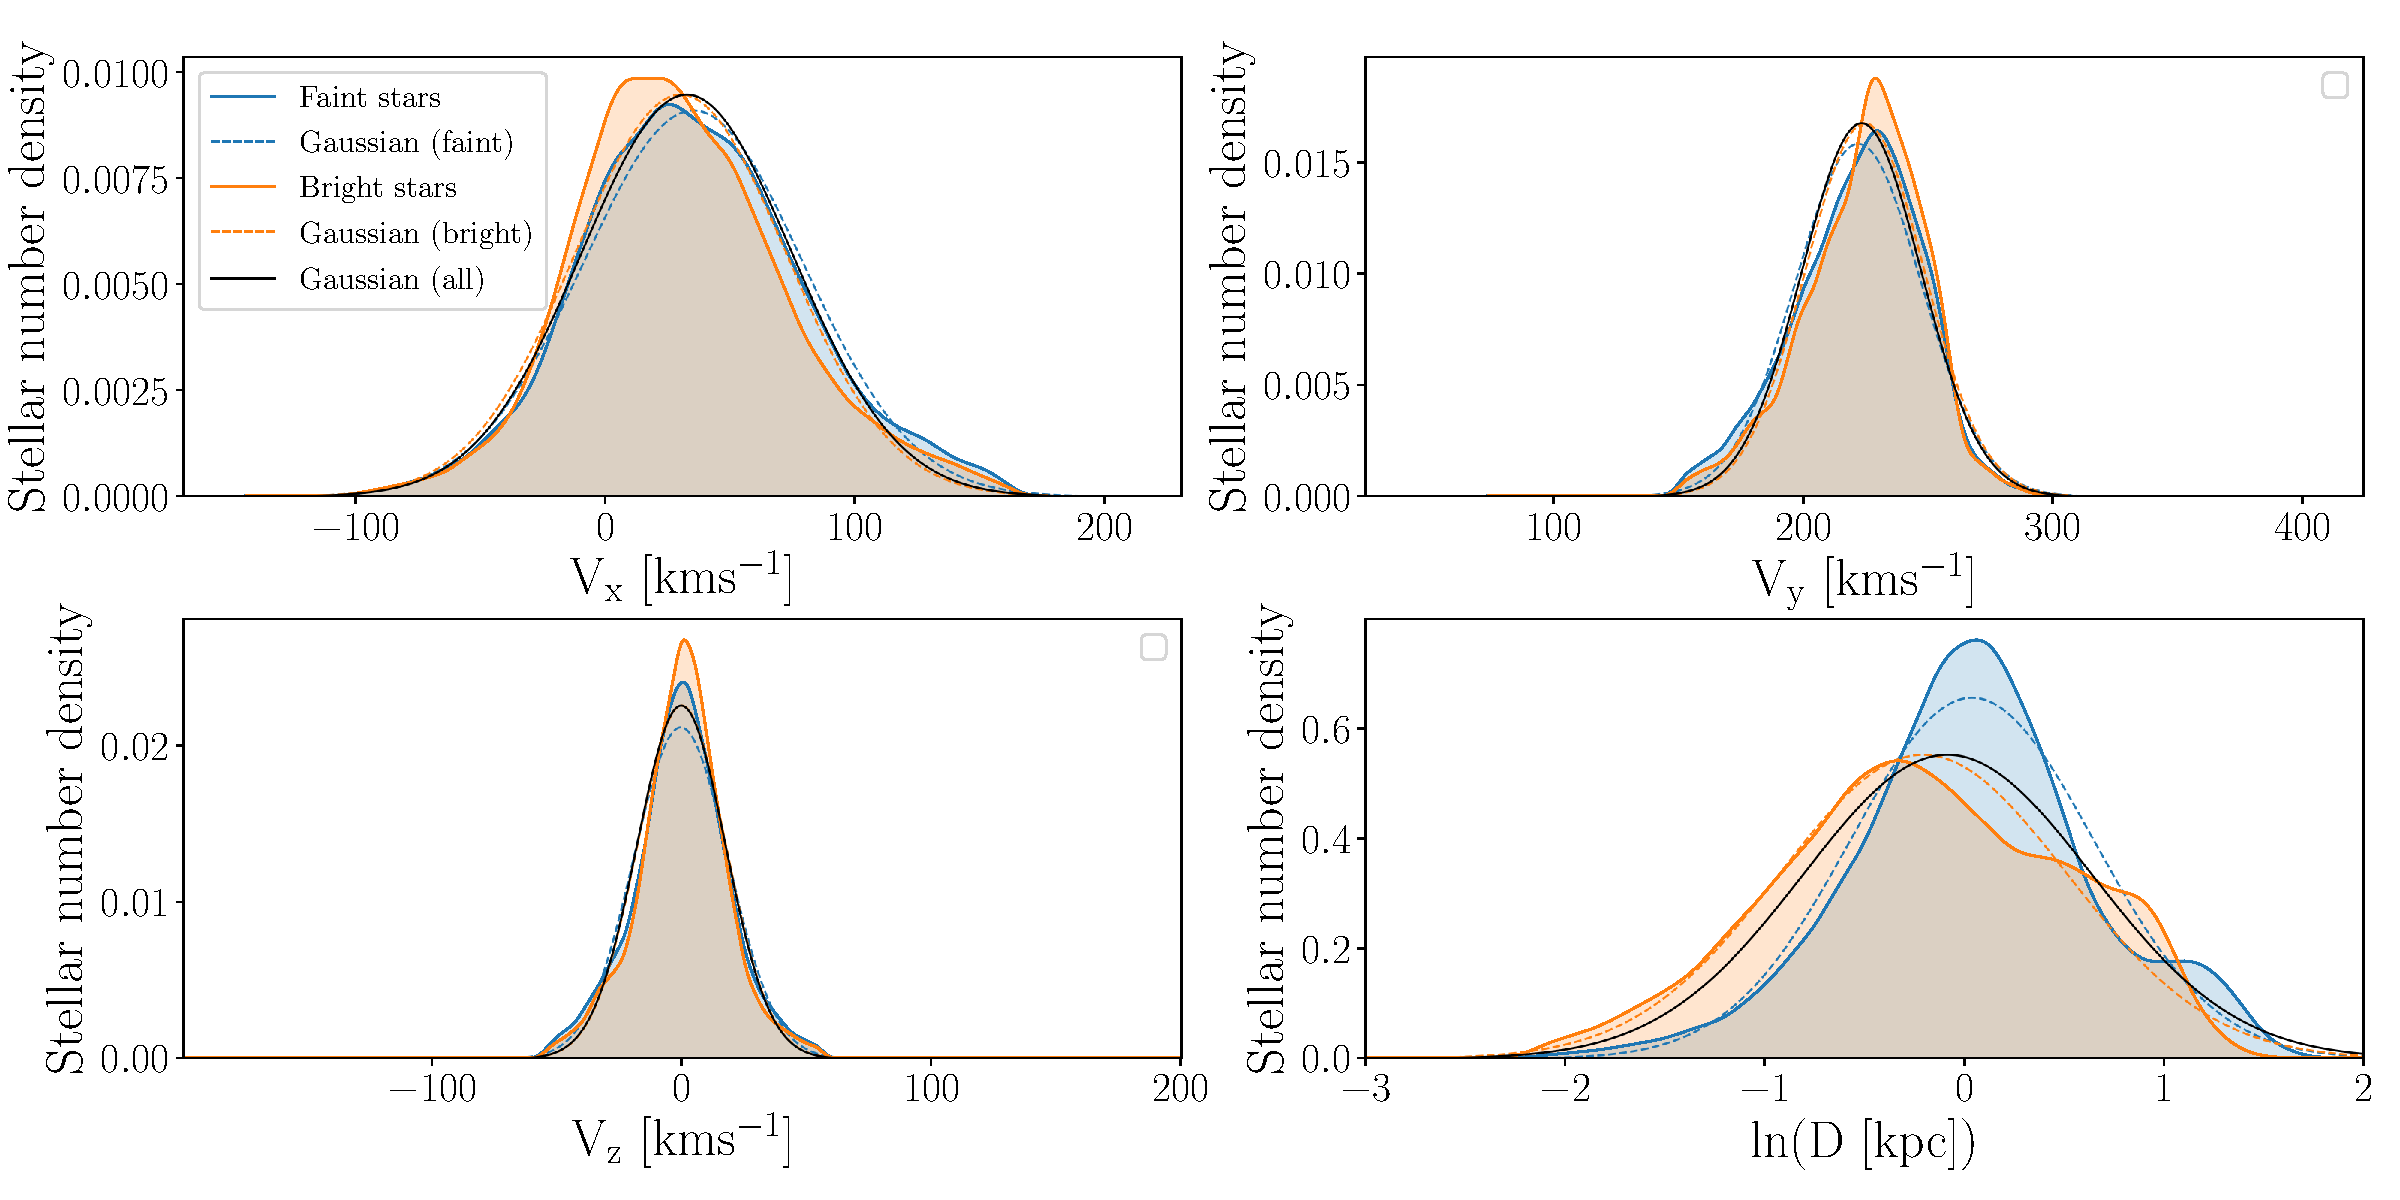
\includegraphics[width=1\textwidth]{prior_distributions}
\label{fig:prior_distributions}
\end{figure}
We inferred the velocities of 3000 stars chosen at random from the
RV Kepler sample using each of these three priors and compared the
inferred velocity distributions.
If the inferred velocities were highly prior-dependent, the resulting
distributions, obtained from different priors, would look very different.
The results of this test are shown in figure \ref{fig:prior_comparison}.
From left to right, the three panels show the distributions of inferred \vx,
\vy, and \vz.
The blue dashed line shows a KDE, representing the distributions of velocities
inferred using the prior calculated from the faint half of the RV sample.
Similarly, the solid orange line shows the distribution of inferred velocities
using the prior calculated from the bright half of the RV sample, and the
solid black line shows the results of the prior calculated from {\it all}
stars with measured RVs.

The median values of the \vy\ distributions, resulting from the faint and
bright priors, differ by around 4 \kms.
This is similar to the difference in means of the faint and bright populations
(5 \kms, as quoted above).
The inferred \vx\ and \vz\ distributions differ by 2 \kms\ and 0.3 \kms,
respectively.
Regardless of the prior choice, the \vx\ and \vz\ distributions are similar
because velocities in the \x\ and \z-directions are not strongly prior
dependent: they are tightly constrained with proper motion measurements alone.
However, the distribution of inferred \vy\ velocities {\it does} depend on the
prior.
This is because the \y-direction is close to the radial direction for \kepler\
stars (see figure \ref{fig:kepler_field}), and \vy\ cannot be tightly
constrained without an RV measurement.
% It is therefore highly dependent on the prior.
\begin{figure}[ht!]
\caption{
The distributions of velocity and distance parameters, inferred using three
    different priors.
The orange line is a KDE that represents the distribution of parameters
    inferred with a Gaussian prior, estimated from the bright half of the RV
    sample ($G < $ 13.9).
The blue dashed line shows the results from a prior estimated from the faint
    half of the RV sample ($G > 13.9$.
The black line shows the results from a prior calculated from all stars with
    RV measurements and is the prior we adopt in our final analysis.
    }
  \centering
    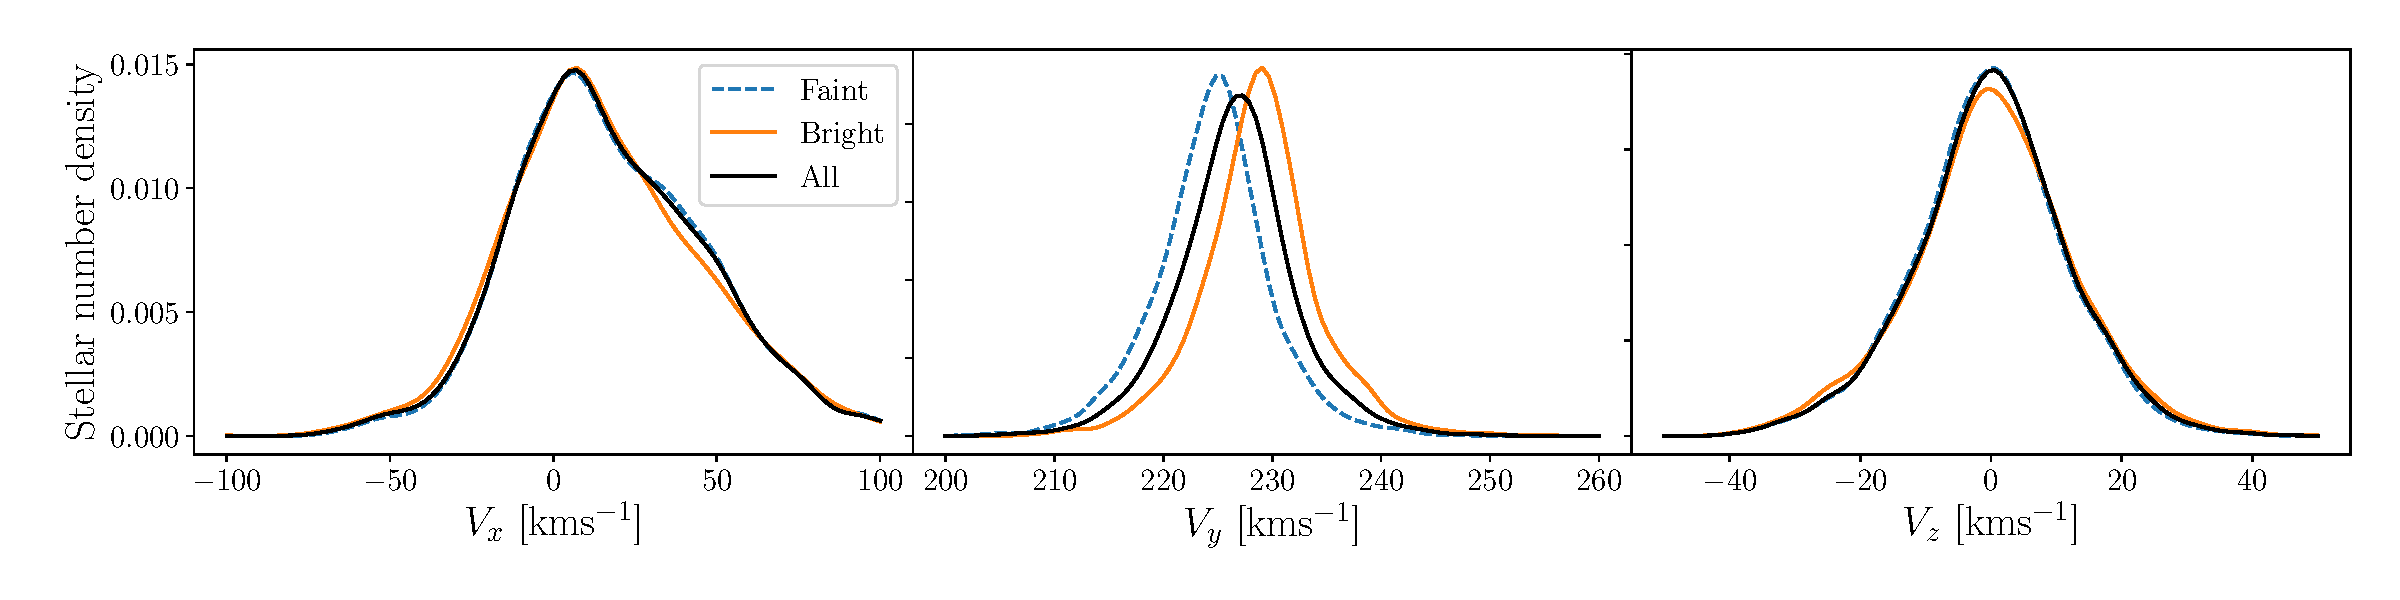
\includegraphics[width=1\textwidth]{prior_comparison}
\label{fig:prior_comparison}
\end{figure}

% Fainter stars have smaller y-velocities than brighter stars because they are,
% on average, further from the Sun

Although this test was performed on stars with RV measurements, which are
brighter overall than the sample of stars without RVs (\eg\ figure
\ref{fig:rv_histogram}), figure \ref{fig:prior_comparison} nevertheless shows
that \vx\ and \vz\ are not strongly prior-dependent.
Since this work is chiefly motivated by kinematic age-dating, which mostly
requires vertical velocities, \vz\, we are satisfied with these results.
The difference in the dispersions of \vz\ velocities, calculated with the
three different priors tested above was smaller than 0.5 \kms.
We conclude that the \vx\ and \vz\ velocities we infer are relatively
insensitive to prior choice, and we adopt a prior calculated from the
distributions of all stars with RV measurements (black Gaussians in figure
\ref{fig:prior_distributions}).
The \vy\ velocities are more strongly prior dependent and should be used with
caution.
